\documentclass[usegeometry=true]{scrartcl}
\usepackage[ngerman]{babel}
\usepackage[T1]{fontenc}
\usepackage{lmodern}
\usepackage[utf8]{inputenc}
\usepackage{hyperref}
\usepackage{amssymb}
% Dimensionen bitte nicht ändern. 
\usepackage[left=2cm, right=2cm, top=2cm, bottom=2cm, bindingoffset=1cm, includeheadfoot]{geometry}
%Zeilenabstand bitte nicht ändern
\usepackage[onehalfspacing]{setspace}
\usepackage{graphicx}

\usepackage[backend=biber,style=numeric,]{biblatex}\addbibresource{literatur.bib}

\begin{document}
% ----------------------------------------------------------------------------
\subject{Projektbericht zum Modul Information Retrieval und Visualisierung Sommersemester 2021}
\title{Titel des Dokuments}
%\subtitle{Untertitel}% optional
\author{Marcus Gagelmann}% obligatorisch
%\date{10.9.2021}
\maketitle% verwendet die zuvor gemachte Angaben zur Gestaltung eines Titels
% ----------------------------------------------------------------------------
% Inhaltsverzeichnis:
%\tableofcontents
% ----------------------------------------------------------------------------
% Gliederung und Text:

\section{Einleitung}
Afrika bildet mit einer Größe von mehr als 30 Millionen Quadratkilometern den zweitgrößten Kontinent der Erde. Insgesamt leben dort über 1,3 Milliarden Menschen, was etwa 17,2\% der Weltbevölkerung ausmacht. Wo jedoch Land und Menschen aufeinander treffen, dort sind auch Konflikte nicht weit entfernt. Seid vielen Jahren fällt Afrika solchen sowohl politischen als auch kriegerischen Auseinandersetzungen zum Opfer. Ursachen hierfür könnten die verbreitete Armut, misswirtschaftende Regierungen sowie die wertvollen Ressourcen des Kontinents sein, um nur einige mögliche Gründe zu nennen. Seit 1997 werden diese Konflikte durch das ACLED-Projekt dokumentiert. ACLED steht hierbei für \glqq Armed Conflict Location and Event Data\grqq{}. Die gesammelten Daten werden von ACLED auf ihrer Website (\url{https://acleddata.com/#/dashboard}) frei zugänglich zur Verfügung gestellt.\\

Nach nun beinahe 25 Jahren an Konfliktaufzeichnungen sind mittlerweile sehr große Datenmengen entstanden, welche einem außenstehenden Tabellenbetrachter kaum einen Überblick über das gesamtgeschehen seit dem Aufzeichnungsbeginn geben können. Noch unwahrscheinlicher ist es, dass ein solcher Betrachter allein mithilfe der unaufbereiteten Daten Rückschlüsse auf mögliche Zusammenhänge zwischen den vielen Konflikten ziehen kann. Mit dieser Ausgangslage ist ein Verstehen der tatsächlichen Lage in Afrika anhand der Daten unmöglich. Hierdurch könnten mögliche Maßnahmen zur Verbesserung der Situation des Kontinents weniger effektiv ausfallen, als wenn das volle Potenzial der Daten ausgeschöpft werden würde.\\

Aus diesem Problem ergibt sich die Fragestellung, ob der gewählte Datensatz hilfreiche Aussagen zu Zusammenhängen ermöglicht, welche die Opfer der Konflikte der letzten 25 Jahre betreffen. Das Ziel dieser Arbeit ist deshalb die Bereitstellung einer Anwendung, welche eine Analyse der Todesopferanzahlen der Afrikakonflikte ermöglicht.

\subsection{Anwendungshintergrund}
Mithilfe der im Rahmen dieser Arbeit entwickelten Anwendung werden einzelne Konflikte für einen Gesamtüberblick über eine oder mehrere Regionen Afrikas zusammengefasst, sowie nach einzelnen Jahren sortiert und hierbei auch mehrdimensional visualisiert. Insgesamt umfasst das Programm zwei verschiedene Ansichten, welche jeweil eine Menge von Konflikten auf unterschiedliche Art und Weise darstellen. In der Hauptansicht, dem Scatterplot, ist es dem Nutzer möglich einen Überblick über die Konfliktdichte und die Opferzahlen zu unterschiedlichen Zeitpunkten seit Aufzeichnungsbeginn zu erhalten. Die Zweitansicht, welche sich der Technik paralleler Koordinaten bedient, zeigt immer eine Teilmenge der Konflikte der Hauptansicht in jeweils drei Dimensionen. Hier kann der Nutzer einen genaueren Einblick erhalten, in welchem Monat eines Jahres welche Art von Konflikt wie viele Todesopfer forderte. Die Basismenge an Konflikten, welche für die Visualisierungen verwendet wird, ergibt sich aus der Menge aller Konflikte des Datensatzes, welche mithilfe eines Regionenfilters gekürzt wird. Dieser Filter wird vom Nutzer über eine dritte Ansicht in Form eines interaktiven Baumes gesteuert. Hier können sowohl die Konflikte größerer Regionen als auch die Konflikte einzelner Länder Afrikas in die visualisierte Gesamtmenge aufgenommen werden.

\subsection{Zielgruppen}
Als Zielgruppe für die Visualisierungsanwendung kommen Personen in Frage, welche einen Überblick über die Konflikt- und Todesopferdichte zu verschiedenen Zeitpunkten und in verschiedenen Regionen des afrikanischen Kontinents erlangen wollen, sowie einen genaueren Einblick in die Art der Konflikte benötigen. Das Programm ist für einen schnellen Einstieg und einen groben Überblick in der Thematik der Afrikakonflikte konzipiert. Aus diesem Grund benötigen Zielgruppen in der Regel kaum Vorwissen um die Anwendung sinnvoll zu nutzen. Politisches und geografisches Vorwissen kann in manchen Anwendungsgebieten für das weitere Verständnis sinnvoll sein, ist aber keines Falls Voraussetzung um Erkenntnisse aus den Daten mithilfe der Anwendung zu gewinnen.\\

Die Verwendung einer solchen Anwendung ist bei Hilfsorganisationen zur Planung zukünftiger Einsätze denkbar. Hiermit könnten zukünftig diejenigen Regionen Afrikas ermittelt werden, welche langfristig die größten Opfer zu beklagen haben und aufbauend auf diesen Fakt weitere Hilfsleistungen am dringensten benötigen. Weiterhin können Hilfskräfte leicht einen Eindruck von der Art der bisherigen Konflikte einer bestimmten Region bekommen und damit zukünftige Einsätze besser auf diese Art von Konflikten vorbereiten.\\

Ein weiteres Anwendungsgebiet könnte die Risikoeinschätzung für Reisen durch das Auswärtige Amt (Link) darstellen. Hier bietet die Anwendung die Möglichkeit, die Gefahr für deutsche Reisende in Konfliktbelasteten Regionen Afrikas besser beurteilen zu können. Gäbe es in den letzten Jahren eine hohe Dichte an politischen Unruhen oder Todesopfer durch Kampfhandlungen, so können hierdurch Urlaubs- und Durchreisende rechtzeitig vor Gefahren gewarnt werden.

\subsection{Überblick und Beiträge}
Dieses Projekt setzt sich zusammen aus dem Datensatz des ACLED-Projekts von 1997-2021 und drei unterschiedlichen Visualisierungstechniken, welche interaktiv miteinander verbunden wurden. Vom verwendete Datensatz werden insgesamt sechs Felder jedes Datenobjektes für die Umsetzung der Anwendung genutzt. Hierzu gehören das Jahr sowie das Datum des Konflikts, die Art des Konflikts, die Region sowie das Land in dem ein Konflikt vorgefallen ist und die Anzahl an Todesopfern, welche ein Konflikt forderte. Die in dem Programm verwendeten Visualisierungstechniken beschränken sich auf eine Hauptansicht mit einem Scatterplot und einer umschaltbaren Zweitansicht, welche parallele Koordinaten zur Umsetzung verwendet. Zusätzlich gibt es noch einen Regionsfilter, welcher mithilfe expliziter Bäume anschaulich umgesetzt wurde. Im Scatterplot findet weiterhin die sogenannte X-Ray-Technik Anwendung, welche dem Nutzer Überlagerungen von Punkten aufzeigen kann. \\

Die Beiträge dieses Projekts belaufen sich auf die Auswahl, die Verarbeitung sowie die Visualisierung von Daten der Konflikte in Afrika in den Jahren 1997 bis 2021. Ganz konkret wird hierbei der Prototyp einer möglichen Anwendung diskutiert, welcher dem Nutzer die gewählten Daten und deren Zusammenhänge als interaktiv verbundenes System näher bringen soll. Hierbei werden die einzelnen Teile der Anwendung kritisch betrachtet, gelungene Ansätze hervorgehoben und Vorschläge zur weiteren Verbesserung geäußert.

\section{Daten}
\begin{figure}[]
\begin{center}

\begin{tabular}{lllll}
 \parbox{5.5cm}{
 \begin{enumerate}
  \item ISO
  \item EVENT\_ID\_CNTY
  \item EVENT\_ID\_NO\_CNTY
  \item EVENT\_DATE
  \item YEAR
  \item TIME\_PRECISION
  \item EVENT\_TYPE
  \item SUB\_EVENT\_TYPE
  \item ACTOR1
  \item ASSOC\_ACTOR\_1
 \end{enumerate}}
 &
 \parbox{4.5cm}{
 \begin{enumerate}
 \setcounter{enumi}{10}
  \item INTER1
  \item ACTOR2
  \item ASSOC\_ACTOR\_2
  \item INTER2
  \item INTERACTION
  \item REGION
  \item COUNTRY
  \item ADMIN1
  \item ADMIN2
  \item ADMIN3
 \end{enumerate}}
 &
 \parbox{5cm}{
 \begin{enumerate}
 \setcounter{enumi}{20}
  \item LOCATION
  \item LATITUDE
  \item LONGITUDE
  \item GEO\_PRECISION
  \item SOURCE
  \item SOURCE\_SCALE
  \item NOTES
  \item FATALITIES
  \item TIMESTAMP
 \end{enumerate}}

\end{tabular}

\caption{Dimensionen des ACLED-Datensatzes}
Quelle: Eigene Darstellung
\label{dimensions}
\end{center}
\end{figure}

Der Datensatz des ACLED-Projekt für die Afrikakonflikte von 1997 bis 2021 beinhaltet insgesamt 65443 einzelne Datenobjekte bzw. Datenzeilen, welche jeweils einen gesonderten Konflikt repräsentieren. Jedes Datenobjekt des Datensatzes liegt in insgesamt 29 Dimensionen vor, welche im einzelnen in Abbildung \ref{dimensions} eingesehen werden können. Verwendet werden von diesen Dimensionen in der Anwendung EVENT\_DATE, YEAR, EVENT\_TYPE, REGION, COUNTRY und FATALITIES. Diese gewählten Dimensionen beinhalten alle für das Programm benötigten Daten und bieten den Vorteil, unkodiert und fast ausschließlich in direkt verwendbarer Form vorzuliegen. Direkt verwendbar bedeutet hierbei, dass die Dimensionen keine weitere Verarbeitung benötigen und direkt in einfach Elm-Datenstrukturen (Int und String) umgewandelt werden können. Lediglich die Dimension EVENT\_DATE bedarf einer zusätzlichen Übersetzerfunktion, welche genutzt werden kann, um den erhaltenen Event-Date-String auf den zugehörigen Monat zu mappen.\\

Es bleibt die Frage, in wie weit sich der Datensatz des ACLED-Projekts für die Zielgruppen dieser Arbeit eignet. Die eindeutigen Daten zu Zeitpunkt, Name des Landes und Todesopfern eignen sich gut für Hilfsorganisationen, um zu ermitteln, welche Länder aktuell am meisten unter den Konflikten leiden. Hierdurch kann eine Vorauswahl getroffen werden, welche Länder momentan Hilfsleistungen benötigen könnten. Mithilfe der Art des Events (EVENT\_TYPE) kann es diesen Organisationen weiterhin gut möglich gemacht werden, die Problemlage im Land besser zu verstehen und einen potenziellen Hilfseinsatz präziser auf eine bestimmte Art von Konflikten vorzubereiten. Bei der Aufgabe einer Gefahreneinschätzung für Reisende durch das Auswärtige Amt kann mithilfe der gewählten Dimensionen des Datensatzes durchaus auch geholfen werden. Informationen wie die Konfliktdichte, die Todesopferdichte und auch die Konfliktarten in einer bestimmten Region lassen eine erste Einschätzungen zu der Situation eines Landes und zur Gefahr für Reisende zu.\\ Eine Verwendung der vorhandenen Geodaten zur Erweiterung der Anwendung durch eine interaktive Karte wäre durchaus denkbar und würde den Zielgruppen beim Verstehen von Zusammenhängen zwischen den Geodaten und den Konfliktdaten zusätzlich helfen. Eine solche Anwendung der Geodaten würde jedoch aufgrund von Problemen bei der Datenaufbereitung (siehe \ref{koordinatenproblem}) sowie der nötigen Ergänzung des Projektes durch Polygondaten für Länderumrisse den Rahmen dieser Arbeit sprengen.\\ Es ist an dieser Stelle wichtig anzumerken, dass die Daten, welche im Programm Anwendung finden, nicht allein ausreichen um die genannten Aufgaben der Zielgruppen zu erfüllen. Da sowohl die Planung von Hilfseinsätzen, als auch die Einschätzung von Gefahrenländern Auswirkungen auf die Sicherheit von Menschenleben haben kann, ist eine Ergänzung des Datensatzes durch zusätzliche detaillierte Informationen zur Politik, Mentalität, Religion und anderen landes- und regionsspezifischen Informationen abseits der aufgezeichneten Konflikte unabdingbar. Beispielsweise kann offen gezeigte Homosexualität momentan in der Republik Kongo zu willkürlichen Verhaftungen wegen angeblich sittenwidrigen Verhaltens führen (\url{https://www.auswaertiges-amt.de/de/aussenpolitik/laender/kongorepublik-node/kongorepubliksicherheit/208542#content_1}), was unbedingt bei einer Gefahreneinschätzung des Landes für westliche Reisende berücksichtigt werden sollte. Diese Information könnte jedoch nicht aus dem gewählten Datensatz ermittelt werden, da sich dieser lediglich auf größere Konflikte und nicht auf einzelne Verhaftungen innerhalb der Republik Kongo stützt.

\subsection{Technische Bereitstellung der Daten}

Bereitgestellt werden die verwendeten Daten von Kaggle (url{https://www.kaggle.com/}), einer Plattform auf der unter anderem Datensätze für Data-Science-Projekte geteilt werden können. Eine andere Möglichkeit für den Download der Daten bietet die Seite des ACLED-Projekts (url{https://acleddata.com/data-export-tool/}). In dieser Arbeit wird der Datensatz von Kaggle verwendet, da die dort bereitgestellten Daten, anders als auf der ACLED-Seite, bereits nach Konflikten im Raum Afrika gefiltert sind. Läd man den Datensatz direkt von Kaggle herunter, so erhält man diesen im CSV-Dateiformat. Als Seperator werden hierbei Semikolons verwendet. Die größe des Datensatzes beläuft sich auf etwa 30,5 MB (30.565.061 Bytes) im Standard CSV-Format, welche sich jedoch auf 62,4 MB (65.467.818 Bytes) mehr als verdoppelt nach einer Umwandlung der Daten in ein JSON-Dateiformat. Die Notwendigkeit für eine solche Umwandlung des Formats wird im Kapitel \ref{sec:datenvorverarbeitung} genauer besprochen.\\ Jede Dimension des Datensatzes ist grundsätzlich entweder als Integer-Wert (Ziffern ohne Komma oder Anführungszeichen) oder als String-Wert (Zeichenfolgen in Anführungszeichen) gegeben. Hierzu gehören auch die Werte LATITUDE und LONGITUDE, welche eigentlich Float-Werte darstellen sollten. Dies stellt ein Problem, welches vor der eigentlichen Verwendung der Daten beim Einlesen durch eine Aufbereitung behoben werden müsste. Die Angaben in LATITUDE und LONGITUDE liegen als String vor, welcher unterschiedlich lange Ziffernfolgen enthalten kann. Hierbei ist keine Kommastelle angegeben, wodurch die Koordinaten des Konflikts nicht eindeutig wiedergegeben werden. Beispielsweise existiert ein Konflikt mit dem Breitengrad 36672 und dem Längengrad 2789. Mit diesen Daten könnten die Koordinaten (3.6672, 27.89) gemeint sein, welche eine Position im Wald in der Demokratischen Republik Kongo bestimmen. Aufgrund der Größe des Kontinents könnten hier jedoch auch die Koordinaten (36.672, 2.789) in Frage kommen, welche eine Position in der Stadt Koléa in Algerien beschreiben. In diesem Fall ist die zweite Möglichkeit korrekt. Es wird jedoch ersichtlich, dass die Position des Kommas in den Breiten- und Längengraden nicht trivial bestimmt werden kann. Einige weitere Dimensionen des Datensatzes sind ebenfalls nicht sehr leicht zugänglich. Die Dimension INTERACTION liegt beispielsweise, neben einigen anderen, nur als numerischer Code vor. Um die tatsächliche Art der Interaktion der betroffenen Parteien ermitteln zu können, müsste hierfür vorher ein Übersetzer mithilfe des Codebooks des ACLED-Projekts (\url{https://reliefweb.int/sites/reliefweb.int/files/resources/ACLED_Codebook_2017FINAL%20%281%29.pdf}) gebaut werden. Das Feld EVENT\_DATE, welches tatsächlich im Programm verwendet wird, besitzt ebenfalls eine erwähnenswerte Formatierung. Die Datumsangaben liegen nämlich im Format \glqq TT-MMMMM-JJJJ\grqq{} vor, wobei der Monat in französischer Sprache ausgeschrieben wird. Hier werden an späterer Stelle (siehe Datenvorverarbeitung) weitere Datenverarbeitung nötig sein. Zuletzt bietet der gewählte Datensatz noch Metadaten, welche sich in die ungekennzeichnet in die anderen Datenfelder einordnen. Hierzu gehören die Dimensionen wie TIME\_PRECISION, welche einen Code für die Genauigkeit der Zeitangaben dieses Datenobjektes angibt und GEO\_PRECISION, welche einen Code für die Genauigkeit der Positionsangaben dieses Datenobjektes angibt. Auch diese müssten bei Bedarf mithilfe eines Übersetzers ausgelesen werden und anschließend zur Umwandlung einer Position/eines Zeitpunktes in einen Bereich/einen Zeitraum verwendet werden.\\

\subsection{Datenvorverarbeitung} \label{sec:datenvorverarbeitung}
Im Rahmen dieses Projektes wurde die Entscheidung getroffen, den vorliegenden CSV-Datensatz in ein entsprechendes JSON-Dateiformat umzuwandeln. Zum einen bietet das JSON-Dateiformat den Vorteil für den Menschen besser lesbar zu sein, was sich als Hilfe bei manuellen Auswertungen während der Entwicklung des Programms herausstellte. Weiterhin werden bei der konvertierung in das JSON-Format Objektstrukturen erstellt und im Datensatz gespeichert, welche von Elm beim Einlesen der Daten direkt in Records übersetzt werden können. Würde der Datensatz als CSV eingelesen werden, so müsste Elm zuerst die gesamte Datei als Zeichenkette einlesen und diese anschließend, aufgrund der fehlenden Objektstrukturen, aufwändiger während der Laufzeit parsen.\\ Beim Start des Programms müssen initiale Datenvorverarbeitungschritte durchgeführt werden, um den View-Funktionen alle nötigen Daten zur korrekten Visualisierung bereistellen zu können. Hierzu gehört eine Initalfilterung der Regionen und Länder, um eine hilfreiche Startansicht gewährleisten zu können. Für diese Startansicht werden alle Konflikte herangezogen, welche sich seit 1997 im Land Ghana zugetragen haben. Hierfür wird die Funktion filterConflicts verwendet, welcher eine Liste aller Konflikte sowie alle aktiv geschalteten Länder und Regionen übergeben werden. Anschließend wird mithilfe der aktiven Länder und Regionen eine Liste derjenigen Länder erstellt, welche letztendlich angezeigt werden sollen. Dies ist wichtig, da in diesem Schritt auch die Länder ganzer aktiver Regionen zur ursprünglichen Liste aktiver Länder hinzu kommen können. Letztendlich wird mithilfe der resultierenden Liste aktiver Länder die Liste aller Konflikte gefiltert. Hierbei werden alle Konflikte beibehalten, dessen Ländername mit einem Land aus der Liste aktiver Länder übereinstimmt.\\ Zusätzlich zur initialen geografischen Filterung müssen auch die französischen Datumsangaben der Dimension EVENT\_DATE mit Tag, Monat und Jahr in die benötigten englische Monatsangaben übersetzt werden. Eine Übersetzung in ein auf den Tag genaues Datum wäre an dieser Stelle ebenfalls denkbar. Monatsangaben reichen hierbei jedoch von der präzision her aus, um den Überblick innerhalb der parallelen Koordinaten (siehe später!!!) zu bewahren. Da die Dimension EVENT\_DATE als String gegeben wird und die französischen Monatsnamen nicht variieren reicht hier eine einfach Übersetzerfunktion aus, welche einen EVENT\_DATE-String auf die französischen Monatsnamen durchsucht und den zugehörigen englischen Monatsnamen zurück gibt. Mithilfe dieser Funktion kann anschließend eine Liste aller EVENT\_DATE-Strings für die weitere Verwendung zu einer Liste mit englischen Monatsbezeichnungen gemappt werden.\\ Für die Visualisierung aller Konflikte eines einzelnen Jahres in der Zweitansicht als parallele Koordinaten wurde unter anderem die EVENT\_TYPE-Dimension in der Anwendung dieses Projektes herangezogen. Hier wurde jedoch bewusst darauf verzichtet die untergeordnete SUB\_EVENT\_TYPE-Dimension ebenfalls zu visualisieren. Durch die Verwendung dieser Dimension würde die Zweitansicht des Programm zwar theoretisch einen höheren Detailgrad an Informationen zu den konkreten Geschehnissen eines Konflikts vermitteln. Es existieren jedoch 23 verschiedene Ausprägungen der SUB\_EVENT\_TYPE-Dimension, wodurch ein Nutzer bei Verwendung dieser Dimension leicht den Überblick verlieren könnte. Da jede einzelne Ausprägung dieser Dimension als relativ lange Zeichenkette in die Visualisierung eingebracht werden müsste, könnten sogar Überlagerungen der Achsenbeschriftungen auftreten. Eine Reduktion des Darstellungsaufwands ist an dieser Stelle keine Möglichkeit, weil jede einzelne Ausprägung der SUB\_EVENT\_TYPE-Dimension eine recht komplexe Information vermittelt, welche nur schwer abgekürzt werden kann. Ein Beispiel hierfür ist ein SUB\_EVENT\_TYPE des EVENT\_TYPE \glqq Battles\grqq{}, welcher mit \glqq Non-state actor overtakes territory\grqq{} bezeichnet wird.\\

\section{Visualisierungen}
\subsection{Analyse der Anwendungsaufgaben}

Insgesamt werden im Rahmen dieser Arbeit zwei Anwendungsaufgaben betrachtet. Zuerst soll die Anwendung Hilfskräften, welche zukünftige Einsätze in Afrika planen, einen schnellen aber gut verständlichen Überblick über die betroffensten Länder aktueller Konflikte verschaffen. Zusätzlich sollte es Mitarbeitern von Behörden wie dem Auswärtigen Amt mithilfe des Programms möglich sein, die Gefahrenlage für Reisende der westlichen Welt einschätzen zu können.\\

Für die erste Aufgabe ist es wichtig, dass die Zielgruppe gezielt Regionen und Länder auf die zugehörige Todesopferdichte untersuchen kann. Weiterhin sollten die Nutzer des Programms in der Lage sein, die am häufigsten vorkommenden Konfliktarten prüfen zu können. Diese Informationen sind nötig, um eingrenzen zu können, welche Regionen und Länder zusätzliche Hilfeleistungen am dringensten benötigen. Weiterhin ist es Nötig die durchschnittliche Anzahl an Todesopfern bei einem Konflikt eines bestimmten Landes oder einer Region einschätzen zu können, um die quantität der zukünftigen Hilfseinsätze festzulegen. Zuletzt ist ein Überblick über die häufigsten Konfliktarten notwendig, damit Hilfsorganisationen einschätzen können, ob und wie viele Sicherheitskräfte einen eventuellen Hilfseinsatz begleiten müssen.\\ Die nötigen genannten Informationen können zum Teil aus der Anwendung gewonnen werden. Beispielsweise hilft der Scatterplot in Verbindung mit dem Regionsfilter beim Aufbau eines mentalen Modells zur Todesopferdichte der verschiedenen Regionen in den letzten Jahren. Hierbei verinnerlicht der Nutzer einen Eindruck von denjenigen Jahren, in denen sich besonders viele Konflikte überlagern, sowie einzelnen \glqq ausreißenden\grqq{} Konflikten, welche eine besonders Hohe Anzahl an Todesopfern forderten. Mithilfe von Parallelen Koordinaten können anschließend einzelne Jahre noch präziser betrachtet werden, um den ersten Überblick über die Opfer dieses Jahres zu festigen und grob einschätzen zu können, welche Art von Konflikten die meisten Opfer forderte. Kritisch betrachtet werden sollte die Fähigkeit der Anwendung, die durchschnittliche Todesopferanzahl eines Jahres zu vermitteln. Mithilfe der verwendeten X-Ray-Technik des Scatterplots sind zwar Konflikthäufungen auszumachen, eine genaue Einschätzung des Todesopferdurchschnitts ist jedoch durch die Verwendung absoluter Zahlen und Überlagerungen nur bedingt möglich. Hier sollte entweder die Anwendung mithilfe weitere Ansichten ausgebaut, oder externe Quellen zur Ergänzung des Programms herangezogen werden. Nicht nötig sind für diese Anwendungsaufgabe die Jahre, welche sich bereits weit in der Vergangenheit befinden. Hier können keine Informationen abgelesen werden, welche aktuelle Hilfseinsätze beeinflussen würden.\\

Für die Aufgabe der Gefahreneinschätzung durch das Auswärtige Amt, welche die Anwendung unterstützen soll, wird ein ähnliches mentales Modell wie für die erste Anwendungsaufgabe benötigt. Hier ist ein breiter Überblick über die Konfliktdichte eines Landes in den letzten Jahren wichtig, um effizient Kandidaten unter den Ländern auszumachen, welche anschließend gründlich auf eine potenzielle Einreisewarnung untersucht werden müssen. Für diese Anwendungsaufgabe könnten weit vergangene Jahre ebenfalls interessant sein, um die Konfliktgeschichte eines Landes besser nachempfinden zu können und damit das zukünftige Gefahrenpotenzial besser einschätzen zu können.\\

\subsection{Anforderungen an die Visualisierungen}
Im Rahmen dieser Arbeit soll eine Anwendung entstehen, welche eine unterstützenden Rolle bei Analysen der Afrikakonflikte von 1997-2021 einnimmt. Die Hauptanforderung an das Programm ist hierfür, dem Nutzer einen schnellen aber effektiven Überblick darüber zu geben, welche Regionen Afrikas besonders von Konflikten geprägt sind und welche Todeszahlen sich hieraus im Vergleich zu anderen Regionen ergeben. Zu diesem Zweck sollten die unterschiedlichen Visualisierungsansichten des Programms in einem relativ \glqq leichten\grqq{} Design gehalten werden. Eine Überzahl an gleichzeitig gezeigten Informationen könnte zwar den Detailgrad der Anwendung erhöhen, der eigentliche Sinn der Anwendung würde hierdurch jedoch in den Hintergrund gerückt werden.\\ Die Filterfunktion für Regionen und Länder ist einer der wichtigsten Teile der Anwendung und bedarf besonderer Sorgfalt bei der Entwicklung. Dem Nutzer muss es möglich sein, flexibel einzelne Länder und ganze Regionen Afrikas zum Filter für die anderen Visualisierungen hinzuzufügen. Zusätzlich sollten Nutzer der Anwendung jeder Zeit Feedback dazu bekommen, welche Konflikte aus welchen Ländern und Regionen ihm momentan angezeigt werden. Zuletzt ist es für den Nutzer durchaus sinnvoll, permanent die geografischen Zusammenhänge zwischen den filterbaren Ländern und Regionen vermittelt zu bekommen, um einen besseren Überblick über aktuelle Filtereinstellungen und deren Bedeutung zu bewahren (siehe später !!!).\\ Die Hauptaufgabe der Anwendung ist die Vermittlung eines Eindrucks der schwere von Konflikten in verschiedenen Ländern und Regionen. Zu diesem Zweck sollte unbedingt eine Darstellung der Opferzahlen in relation zu unterschiedlichen sinnvollen Dimensionsausprägungen erfolgen, um einzelne Ereignisse, ganze Länder und Länderübergreifende Regionen zu einem bestimmten Zeitpunkt besser zu verstehen. Hierfür bieten sich beispielsweise Zeiteinheiten, Konfliktarten oder auch Geodaten an. Die Verwendung der Jahresdaten ist in diesem Fall besonders entscheidend für die Zielgruppen, um aktuelle Ereignisse von weit vergangenen unterscheiden zu können. Die genauere Untersuchung einzelner Jahre als \glqq visualisierter Ausschnitt\grqq{} könnte hierbei von Vorteil sein.\\

\subsection{Präsentation der Visualisierungen}
Präsentieren sie die visuelle Abbildungen und Kodierungen der Daten und Interaktionsmöglichkeiten. 
Sie müssen  begründen, warum und wiegut ihre Designentscheidungen die erstellten Anforderungen erfüllen. 
Weiterhin müssen sie begründen, warum die gewählte visuelle Kodierung der Daten für das zulösenden Problem passend ist. 
Typische Argumente würden hier auf Wahrnehmungsprinzipien und Theorie über Informationsvisualisierung verweisen. 
Die besten Begründungen diskutieren explizit die konkrete Auswahl der Visualisierungen im Kontext von mehreren verschiedenen Alternativen. Diskutieren sie die Expressivität und die Effektivität der einzelnen Visualisierungen.

Die eben beschriebenen Präsentationen und Begründungen sollen für jede der drei folgenden Visualisierungen durchgeführt werden. 
\subsubsection{Visualisierung Eins}

\begin{figure}[]
\begin{center}
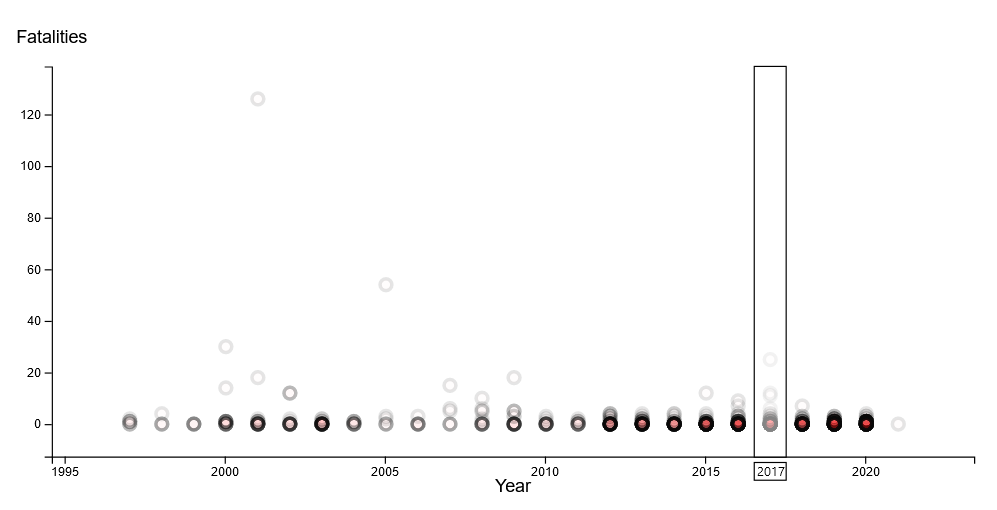
\includegraphics[width=12cm,height=10cm,keepaspectratio]{Scatterplot.PNG}%
\caption{Screenshot eines möglichen Scatterplots}
Quelle: Eigene Darstellung
\label{scatterplot}
\end{center}
\end{figure}

Die erste Visualisierung innerhalb der Anwendung ist in Abbildung \ref{scatterplot} zu sehen und zeigt einen zweidimensionaler Scatterplot, welcher sowohl die Dimension der Todesopferanzahlen (\glqq Fatalities\grqq{}) als auch die zugehörigen Jahre darstellt. Hierbei werden die Achsen dynamisch an die aktuell angezeigten Daten angepasst, um diese immer maximal auf die zur Verfügung stehende Fläche zu verteilen. Jeder Datenpunkt in der Visualisierung stellt einen Konflikt des ACLED-Datensatzes dar. Diese werden in der Darstellung mit einer hohen transparenz angezeigt, um einen X-Ray-Effekt zu erzeugen, wodurch Überlappungen leicht erkannt werden können. Das Design der Datenpunkte ist geprägt durch einen dicken schwarzer Ring mit einer hohen transparenz (alpha-Wert von 0.1), welcher mit einem Rotton gefüllt ist, der nochmal um ein zehnfaches transparenter ist (alpha-Wert von 0.01). Das letzte Detail der Scatterplot-Visualisierung ist das interaktive Feature der Jahresauswahl. Hierfür wird der Scatterplot in gedachte Spalten eingeteilt, welche an Jahresachse ausgerichtet sind. Durch einen Hover der Maus über eine dieser Spalten erscheint für die Dauer des Hovers ein Spaltenumfassendes Rechteck mit schwarzen Rändern und stark transparenter weißer Füllung. Zusätzlich erscheint auf der Jahresachse das betreffende, schwarz umrandete Jahr für die Dauer des Maus-Hovers. Ein klick auf eine der markierten Flächen lässt die Anwendung in die zweite Visualisierung (siehe !!!) des ausgewählten Jahres wechseln.\\ Die Anforderung an die Visualisierung, einen ersten schnellen Überblick über die Todesopferzahlen der angezeigten Regionen zu gewähren, wird von der ersten Ansicht größtenteils erfüllt. Grund hierfür ist das minimalistische aber leicht verständliche Design, welches auf der allgemein bekannten Visualisierungstechnik des zweidimensionalen Scatterplots beruht. Dieser Fakt in Kombination mit nur zwei unterschiedlichen verwendeten Farben ermöglicht es einem Betrachter ohne längere Betrachtungszeit einen Überblick über die präsentierten Informationen zu gewinnen. Der Gehalt der präsentierten Informationen könnte wiederum noch höher sein.\\ Ein Problem der ersten Visualisierung ist die Umsetzung der X-Ray-Technik. Diese vermittelt zwar eindeutig und auf den ersten Blick höhere und weniger hohe Konfliktdichten, wie viele Datenpunkte in solchen Clustern jedoch genau vorhanden sind kann der Betrachter nur schlecht erahnen. Ab einer gewissen Konfliktüberlappung gleichen sich die Cluster zu stark um sie präzise unterscheiden zu können. Dies könnte seinen Ursprung darin haben, dass ein linearer Anstieg des Helligkeitsstimulus nur zu einem sublinearen Zuwachs an wahrgenommener Helligkeit (oder Dunkelheit) korrespondiert (zitat S2S130 ca). In anderen Worten bedeutet das, dass ab einer gewissen Sättigungs- bzw. \glqq Dunkelheitsstufe\grqq{} bei einem Datenpunkte bei gleich bleibender, linearer verdunklung immer weniger Veränderung für das menschliche Auge wahrnehmbar ist. Hier könnte die Anwendung einer Gammakorrektur abhilfe verschaffen, welche die linearen Helligkeitsabstufungen auf eine andere gewünschte Weise skalieren kann. Hiermit könnten auch bei höheren Datenpunktdichten noch wahrnehmbare Unterschiede herbeigeführt werden.\\ Ein weiteres Problem des Scatterplots ist die Verteilung der Datenpunkte auf der Fatalities-Achse. Hier ist bei fast allen möglichen Regionszusammensetzungen zu beobachten, dass sich der Großteil der Datenpunkte im untersten Bereich der Grafik ansammeln. Einzelne Ausreißer lassen die Reichweiter der Fatalities-Achse jedoch bis zu weit überdurchschnittlichen Werten verlaufen. Um die Datenpunkte auf dieser Grundlage besser in der Grafik zu verteilen, könnte hier eine logarithmische statt einer linearen Skalierung der Fatalities-Achse angebracht sein. Hierdurch würden die stark komprimierten Datenpunkte um unteren Ende der Grafik eventuell besser im oberen Bereich verteilt werden. Hierdurch würde zum einen der Platz innerhalb der Grafik besser zur Informationsdarstellung genutzt werden, zum anderen könnte dieser Ansatz ebenfalls beim ersten Problem der zu hohen Datenpunktdichte helfen.\\

\subsubsection{Visualisierung Zwei}
-parallele koord: bild, achsen, datenlinien
-anforderungserfüllung: detailreicher als 1., aber noch nicht zu überladen ->
	monat/art in relation zu todeszahlen gesetzt für besseres verständnis von zeitpunkt und vorkommnis
	"slicing" der daten nach jahr -> kleine konfliktmenge genauer betrachten als visualisierter Ausschnitt des ganzen
	einzelne konflikte bei größeren mengen hier nicht zu verfolgen -> konzentration für einzelne Dimensionsausprägungen erkennbar -> anforderung "überblick" erfüllt, aber ausbaufähig: problem: konflikte die in 2 benachbarten dims gleiche ausprägung haben sehen aus wie eins -> xray könnte abhilfe verschaffen / unterschiedliche farben für typen in scatterplot könnte ebenfalls das problem lösen, solange scala wenige überlappungen zulässt (in aktuellem scatterplot keine lösung)

\subsubsection{Visualisierung Drei}
-baum: bild, ebenen, farbbedeutung, abkürzungen + namenshover

\subsection{Interaktion}
-checkboxes als filter nicht umgesetzt -> bessere übersicht über geografische verhältnisse

Erklären sie die möglichen Interaktionen mit den einzelnen Visualisierungen und die möglichen Verknüpfungen zwischen ihnen. Begründen Sie warum die konkreten Interaktionen umgesetzt wurden und welche Zwecke für die Anwenderinnen mit ihnen unterstützt werden. Begründen sie ebenfalls warum sie andere Interaktionsmöglichkeiten nicht umgesetzt haben. 

\section{Implementierung}
Beschreiben Sie die Implementierung ihrer Visualisierungsanwendung in Elm. Stellen die Gliederung ihres Quellcodes vor. Haben Sie verschiedene Elm-Module erstellt. Was war aufwändig umzusetzen, was ließ sich mit dem vorhanden Code aus den Übungen relativ einfach umsetzen? 

Wie sieht die Elm-Datenstruktur für das Model aus, in dem die verschiedenen Zustände der Interaktion gespeichert werden können.

\section{Anwendungsfälle}
Präsentieren sie für jede der drei Visualisierungen einen sinnvollen Anwendungsfall in dem ein bestimmter Fakt, ein Muster oder die Abwesenheit eines Musters visuell festgestellt wird. Begründen sie warum dieser Anwendungsfall wichtig für die Zielgruppe der Anwenderinnen ist. Diskutieren sie weiterhin, ob die oben beschriebene Information auch mit anderen Visualisierungstechniken hätte gefunden werden können. Falls dies möglich wäre, vergleichen sie die den Aufwand und die Schwierigkeiten ihres Ansatzes und der Alternativen. 
\subsection{Anwendung Visualisierung Eins}
\subsection{Anwendung Visualisierung Zwei}
\subsection{Anwendung Visualisierung Drei}

\section{Verwandte Arbeiten}
Führen sie eine kurze Literatursuche in der wissenschaftlichen Literatur zu Informationsvisualisierung und Visual Analytics nach ähnlichen Anwendungen durch. Diskutieren sie mindestens zwei Artikel. Stellen sie Gemeinsamkeiten und Unterschiede dar.

\section{Zusammenfassung und Ausblick}

-verschiedene Länder/Regionen unterscheiden (z.B. Farben)

Fassen sie die Beiträge ihre Visualisierungsanwendung zusammen. Wo bietet sie für die Personen der Zielgruppe einen echten Mehrwert.

Was wären mögliche sinnvolle Erweiterungen, entweder auf der Ebene der Visualisierungen und/oder auf der Datenebene?

\section*{Anhang: Git-Historie}

\printbibliography

\end{document}

